\PassOptionsToPackage{unicode=true}{hyperref} % options for packages loaded elsewhere
\PassOptionsToPackage{hyphens}{url}
%
\documentclass[]{article}
\usepackage{lmodern}
\usepackage{amssymb,amsmath}
\usepackage{ifxetex,ifluatex}
\usepackage{fixltx2e} % provides \textsubscript
\ifnum 0\ifxetex 1\fi\ifluatex 1\fi=0 % if pdftex
  \usepackage[T1]{fontenc}
  \usepackage[utf8]{inputenc}
  \usepackage{textcomp} % provides euro and other symbols
\else % if luatex or xelatex
  \usepackage{unicode-math}
  \defaultfontfeatures{Ligatures=TeX,Scale=MatchLowercase}
\fi
% use upquote if available, for straight quotes in verbatim environments
\IfFileExists{upquote.sty}{\usepackage{upquote}}{}
% use microtype if available
\IfFileExists{microtype.sty}{%
\usepackage[]{microtype}
\UseMicrotypeSet[protrusion]{basicmath} % disable protrusion for tt fonts
}{}
\IfFileExists{parskip.sty}{%
\usepackage{parskip}
}{% else
\setlength{\parindent}{0pt}
\setlength{\parskip}{6pt plus 2pt minus 1pt}
}
\usepackage{hyperref}
\hypersetup{
            pdftitle={Get start with R},
            pdfauthor={Lea Lai},
            pdfborder={0 0 0},
            breaklinks=true}
\urlstyle{same}  % don't use monospace font for urls
\usepackage[margin=1in]{geometry}
\usepackage{color}
\usepackage{fancyvrb}
\newcommand{\VerbBar}{|}
\newcommand{\VERB}{\Verb[commandchars=\\\{\}]}
\DefineVerbatimEnvironment{Highlighting}{Verbatim}{commandchars=\\\{\}}
% Add ',fontsize=\small' for more characters per line
\usepackage{framed}
\definecolor{shadecolor}{RGB}{248,248,248}
\newenvironment{Shaded}{\begin{snugshade}}{\end{snugshade}}
\newcommand{\AlertTok}[1]{\textcolor[rgb]{0.94,0.16,0.16}{#1}}
\newcommand{\AnnotationTok}[1]{\textcolor[rgb]{0.56,0.35,0.01}{\textbf{\textit{#1}}}}
\newcommand{\AttributeTok}[1]{\textcolor[rgb]{0.77,0.63,0.00}{#1}}
\newcommand{\BaseNTok}[1]{\textcolor[rgb]{0.00,0.00,0.81}{#1}}
\newcommand{\BuiltInTok}[1]{#1}
\newcommand{\CharTok}[1]{\textcolor[rgb]{0.31,0.60,0.02}{#1}}
\newcommand{\CommentTok}[1]{\textcolor[rgb]{0.56,0.35,0.01}{\textit{#1}}}
\newcommand{\CommentVarTok}[1]{\textcolor[rgb]{0.56,0.35,0.01}{\textbf{\textit{#1}}}}
\newcommand{\ConstantTok}[1]{\textcolor[rgb]{0.00,0.00,0.00}{#1}}
\newcommand{\ControlFlowTok}[1]{\textcolor[rgb]{0.13,0.29,0.53}{\textbf{#1}}}
\newcommand{\DataTypeTok}[1]{\textcolor[rgb]{0.13,0.29,0.53}{#1}}
\newcommand{\DecValTok}[1]{\textcolor[rgb]{0.00,0.00,0.81}{#1}}
\newcommand{\DocumentationTok}[1]{\textcolor[rgb]{0.56,0.35,0.01}{\textbf{\textit{#1}}}}
\newcommand{\ErrorTok}[1]{\textcolor[rgb]{0.64,0.00,0.00}{\textbf{#1}}}
\newcommand{\ExtensionTok}[1]{#1}
\newcommand{\FloatTok}[1]{\textcolor[rgb]{0.00,0.00,0.81}{#1}}
\newcommand{\FunctionTok}[1]{\textcolor[rgb]{0.00,0.00,0.00}{#1}}
\newcommand{\ImportTok}[1]{#1}
\newcommand{\InformationTok}[1]{\textcolor[rgb]{0.56,0.35,0.01}{\textbf{\textit{#1}}}}
\newcommand{\KeywordTok}[1]{\textcolor[rgb]{0.13,0.29,0.53}{\textbf{#1}}}
\newcommand{\NormalTok}[1]{#1}
\newcommand{\OperatorTok}[1]{\textcolor[rgb]{0.81,0.36,0.00}{\textbf{#1}}}
\newcommand{\OtherTok}[1]{\textcolor[rgb]{0.56,0.35,0.01}{#1}}
\newcommand{\PreprocessorTok}[1]{\textcolor[rgb]{0.56,0.35,0.01}{\textit{#1}}}
\newcommand{\RegionMarkerTok}[1]{#1}
\newcommand{\SpecialCharTok}[1]{\textcolor[rgb]{0.00,0.00,0.00}{#1}}
\newcommand{\SpecialStringTok}[1]{\textcolor[rgb]{0.31,0.60,0.02}{#1}}
\newcommand{\StringTok}[1]{\textcolor[rgb]{0.31,0.60,0.02}{#1}}
\newcommand{\VariableTok}[1]{\textcolor[rgb]{0.00,0.00,0.00}{#1}}
\newcommand{\VerbatimStringTok}[1]{\textcolor[rgb]{0.31,0.60,0.02}{#1}}
\newcommand{\WarningTok}[1]{\textcolor[rgb]{0.56,0.35,0.01}{\textbf{\textit{#1}}}}
\usepackage{graphicx,grffile}
\makeatletter
\def\maxwidth{\ifdim\Gin@nat@width>\linewidth\linewidth\else\Gin@nat@width\fi}
\def\maxheight{\ifdim\Gin@nat@height>\textheight\textheight\else\Gin@nat@height\fi}
\makeatother
% Scale images if necessary, so that they will not overflow the page
% margins by default, and it is still possible to overwrite the defaults
% using explicit options in \includegraphics[width, height, ...]{}
\setkeys{Gin}{width=\maxwidth,height=\maxheight,keepaspectratio}
\setlength{\emergencystretch}{3em}  % prevent overfull lines
\providecommand{\tightlist}{%
  \setlength{\itemsep}{0pt}\setlength{\parskip}{0pt}}
\setcounter{secnumdepth}{5}
% Redefines (sub)paragraphs to behave more like sections
\ifx\paragraph\undefined\else
\let\oldparagraph\paragraph
\renewcommand{\paragraph}[1]{\oldparagraph{#1}\mbox{}}
\fi
\ifx\subparagraph\undefined\else
\let\oldsubparagraph\subparagraph
\renewcommand{\subparagraph}[1]{\oldsubparagraph{#1}\mbox{}}
\fi

% set default figure placement to htbp
\makeatletter
\def\fps@figure{htbp}
\makeatother


\title{Get start with R}
\author{Lea Lai}
\date{February 23, 2019}

\begin{document}
\maketitle

{
\setcounter{tocdepth}{2}
\tableofcontents
}
\hypertarget{a-start-get-use-to-r}{%
\section{A start: Get use to R}\label{a-start-get-use-to-r}}

(Partially credit to Nicole Kelbick, PhD. and introduction to R
\url{https://cran.r-project.org/doc/manuals/r-release/R-intro.pdf})

Don't afriad to use R. It can be very simple. You can start by open R
and type in only one line, and it will work. Try the following:

(The ones with ** are frequently used)

\hypertarget{common-used-operation-or-funtions}{%
\subsection{Common used operation or
funtions}\label{common-used-operation-or-funtions}}

\hypertarget{section}{%
\subsubsection{** ``:''}\label{section}}

The operator `:' generates a sequence of integers.

\begin{Shaded}
\begin{Highlighting}[]
\DecValTok{1}\OperatorTok{:}\DecValTok{10}
\end{Highlighting}
\end{Shaded}

\begin{verbatim}
##  [1]  1  2  3  4  5  6  7  8  9 10
\end{verbatim}

\begin{Shaded}
\begin{Highlighting}[]
\DecValTok{10}\OperatorTok{:}\DecValTok{1}
\end{Highlighting}
\end{Shaded}

\begin{verbatim}
##  [1] 10  9  8  7  6  5  4  3  2  1
\end{verbatim}

\hypertarget{or}{%
\subsubsection{``\textless{}-'' or ``=''}\label{or}}

You can assign values to variables using `\textless{}-' OR `='.

\begin{Shaded}
\begin{Highlighting}[]
\NormalTok{x <-}\StringTok{ }\DecValTok{5}
\NormalTok{x}
\end{Highlighting}
\end{Shaded}

\begin{verbatim}
## [1] 5
\end{verbatim}

\begin{Shaded}
\begin{Highlighting}[]
\NormalTok{x=}\DecValTok{2}
\NormalTok{x}
\end{Highlighting}
\end{Shaded}

\begin{verbatim}
## [1] 2
\end{verbatim}

\hypertarget{these-are-basic-arithmetic-operations}{%
\subsubsection{``+'' ``-'' "*" ``/'' ``\%\%'' These are basic arithmetic
operations}\label{these-are-basic-arithmetic-operations}}

\begin{Shaded}
\begin{Highlighting}[]
\NormalTok{x}\OperatorTok{+}\DecValTok{5}
\end{Highlighting}
\end{Shaded}

\begin{verbatim}
## [1] 7
\end{verbatim}

\begin{Shaded}
\begin{Highlighting}[]
\NormalTok{x}\OperatorTok{*}\DecValTok{5}
\end{Highlighting}
\end{Shaded}

\begin{verbatim}
## [1] 10
\end{verbatim}

\begin{Shaded}
\begin{Highlighting}[]
\NormalTok{x}\OperatorTok{/}\DecValTok{5}
\end{Highlighting}
\end{Shaded}

\begin{verbatim}
## [1] 0.4
\end{verbatim}

\begin{Shaded}
\begin{Highlighting}[]
\NormalTok{x}\OperatorTok\DecValTok{5} \CommentTok{#give the remainder of x}
\end{Highlighting}
\end{Shaded}

\begin{verbatim}
## [1] 2
\end{verbatim}

\hypertarget{seqfromtospacing}{%
\subsubsection{** ``seq(from,to,spacing)''}\label{seqfromtospacing}}

The `seq' function generates a sequence of numbers with a specified
spacing.\\
seq( from,to,spacing)

\begin{Shaded}
\begin{Highlighting}[]
\NormalTok{xn <-}\StringTok{ }\KeywordTok{seq}\NormalTok{(}\DecValTok{1}\NormalTok{,}\DecValTok{10}\NormalTok{,.}\DecValTok{1}\NormalTok{)}
\NormalTok{xn}
\end{Highlighting}
\end{Shaded}

\begin{verbatim}
##  [1]  1.0  1.1  1.2  1.3  1.4  1.5  1.6  1.7  1.8  1.9  2.0  2.1  2.2  2.3  2.4
## [16]  2.5  2.6  2.7  2.8  2.9  3.0  3.1  3.2  3.3  3.4  3.5  3.6  3.7  3.8  3.9
## [31]  4.0  4.1  4.2  4.3  4.4  4.5  4.6  4.7  4.8  4.9  5.0  5.1  5.2  5.3  5.4
## [46]  5.5  5.6  5.7  5.8  5.9  6.0  6.1  6.2  6.3  6.4  6.5  6.6  6.7  6.8  6.9
## [61]  7.0  7.1  7.2  7.3  7.4  7.5  7.6  7.7  7.8  7.9  8.0  8.1  8.2  8.3  8.4
## [76]  8.5  8.6  8.7  8.8  8.9  9.0  9.1  9.2  9.3  9.4  9.5  9.6  9.7  9.8  9.9
## [91] 10.0
\end{verbatim}

\begin{Shaded}
\begin{Highlighting}[]
\KeywordTok{seq}\NormalTok{(}\DecValTok{1}\NormalTok{,}\DecValTok{10}\NormalTok{,}\DataTypeTok{length.out =} \DecValTok{20}\NormalTok{) }\CommentTok{#use length.out to specify how many you need within the range}
\end{Highlighting}
\end{Shaded}

\begin{verbatim}
##  [1]  1.000000  1.473684  1.947368  2.421053  2.894737  3.368421  3.842105
##  [8]  4.315789  4.789474  5.263158  5.736842  6.210526  6.684211  7.157895
## [15]  7.631579  8.105263  8.578947  9.052632  9.526316 10.000000
\end{verbatim}

\hypertarget{rev}{%
\subsubsection{``rev''}\label{rev}}

The `rev' function reverses values of argument.

\begin{Shaded}
\begin{Highlighting}[]
\NormalTok{yn <-}\StringTok{ }\KeywordTok{rev}\NormalTok{(xn)}
\NormalTok{yn}
\end{Highlighting}
\end{Shaded}

\begin{verbatim}
##  [1] 10.0  9.9  9.8  9.7  9.6  9.5  9.4  9.3  9.2  9.1  9.0  8.9  8.8  8.7  8.6
## [16]  8.5  8.4  8.3  8.2  8.1  8.0  7.9  7.8  7.7  7.6  7.5  7.4  7.3  7.2  7.1
## [31]  7.0  6.9  6.8  6.7  6.6  6.5  6.4  6.3  6.2  6.1  6.0  5.9  5.8  5.7  5.6
## [46]  5.5  5.4  5.3  5.2  5.1  5.0  4.9  4.8  4.7  4.6  4.5  4.4  4.3  4.2  4.1
## [61]  4.0  3.9  3.8  3.7  3.6  3.5  3.4  3.3  3.2  3.1  3.0  2.9  2.8  2.7  2.6
## [76]  2.5  2.4  2.3  2.2  2.1  2.0  1.9  1.8  1.7  1.6  1.5  1.4  1.3  1.2  1.1
## [91]  1.0
\end{verbatim}

\hypertarget{celem1elem2}{%
\subsubsection{** ``c(elem1,elem2)''}\label{celem1elem2}}

The operator 'c'combines different elements into a vector

\begin{Shaded}
\begin{Highlighting}[]
\KeywordTok{c}\NormalTok{(}\DecValTok{1}\NormalTok{,}\DecValTok{2}\NormalTok{)}
\end{Highlighting}
\end{Shaded}

\begin{verbatim}
## [1] 1 2
\end{verbatim}

\begin{Shaded}
\begin{Highlighting}[]
\KeywordTok{c}\NormalTok{(}\StringTok{"1"}\NormalTok{,}\DecValTok{2}\NormalTok{) }\CommentTok{#the same as c("1","2"), they are all stored as strings. }
\end{Highlighting}
\end{Shaded}

\begin{verbatim}
## [1] "1" "2"
\end{verbatim}

\hypertarget{reparg1n}{%
\subsubsection{** rep(arg1,n)}\label{reparg1n}}

`rep(arg1, n)' repeats the first argument (arg1) n times

\begin{Shaded}
\begin{Highlighting}[]
\KeywordTok{rep}\NormalTok{(}\DecValTok{2}\NormalTok{,}\DecValTok{7}\NormalTok{)}
\end{Highlighting}
\end{Shaded}

\begin{verbatim}
## [1] 2 2 2 2 2 2 2
\end{verbatim}

\begin{Shaded}
\begin{Highlighting}[]
\NormalTok{y <-}\StringTok{ }\KeywordTok{c}\NormalTok{(}\DecValTok{1}\NormalTok{, }\DecValTok{3}\NormalTok{, }\FloatTok{5.5}\NormalTok{, }\KeywordTok{rep}\NormalTok{(}\DecValTok{2}\NormalTok{,}\DecValTok{7}\NormalTok{))}
\NormalTok{y}
\end{Highlighting}
\end{Shaded}

\begin{verbatim}
##  [1] 1.0 3.0 5.5 2.0 2.0 2.0 2.0 2.0 2.0 2.0
\end{verbatim}

\begin{Shaded}
\begin{Highlighting}[]
\KeywordTok{rep}\NormalTok{(}\KeywordTok{c}\NormalTok{(}\DecValTok{1}\NormalTok{,}\DecValTok{3}\NormalTok{),}\DecValTok{3}\NormalTok{) }\CommentTok{# repeat 1,3 for 3 times}
\end{Highlighting}
\end{Shaded}

\begin{verbatim}
## [1] 1 3 1 3 1 3
\end{verbatim}

\begin{Shaded}
\begin{Highlighting}[]
\KeywordTok{rep}\NormalTok{(}\KeywordTok{seq}\NormalTok{(}\DecValTok{1}\NormalTok{,}\DecValTok{3}\NormalTok{),}\DecValTok{2}\OperatorTok{:}\DecValTok{4}\NormalTok{) }\CommentTok{# repeat 1,2,3 correspondingly for 2,3,4 times}
\end{Highlighting}
\end{Shaded}

\begin{verbatim}
## [1] 1 1 2 2 2 3 3 3 3
\end{verbatim}

\hypertarget{type-casting-as.numeric-and-etc.}{%
\subsubsection{Type casting: as.numeric and
etc.}\label{type-casting-as.numeric-and-etc.}}

Change string to number; or change number to string

\begin{Shaded}
\begin{Highlighting}[]
\KeywordTok{as.numeric}\NormalTok{(}\StringTok{"1"}\NormalTok{) }\CommentTok{#when you add  " " , the content in the double quotation marks become strings}
\end{Highlighting}
\end{Shaded}

\begin{verbatim}
## [1] 1
\end{verbatim}

\begin{Shaded}
\begin{Highlighting}[]
\KeywordTok{as.character}\NormalTok{(}\DecValTok{1}\NormalTok{)}
\end{Highlighting}
\end{Shaded}

\begin{verbatim}
## [1] "1"
\end{verbatim}

\hypertarget{section-1}{%
\subsubsection{``;''}\label{section-1}}

The operator ``;'' can be used as a seperation for each command when
writing on the same line

\begin{Shaded}
\begin{Highlighting}[]
\KeywordTok{print}\NormalTok{(x);}\KeywordTok{print}\NormalTok{(y)}
\end{Highlighting}
\end{Shaded}

\begin{verbatim}
## [1] 2
\end{verbatim}

\begin{verbatim}
##  [1] 1.0 3.0 5.5 2.0 2.0 2.0 2.0 2.0 2.0 2.0
\end{verbatim}

\hypertarget{meanvarsdmedian}{%
\subsubsection{``mean'';``var'';``sd'',``median''}\label{meanvarsdmedian}}

\begin{Shaded}
\begin{Highlighting}[]
\NormalTok{x=}\DecValTok{1}\OperatorTok{:}\DecValTok{10}\NormalTok{;x}
\end{Highlighting}
\end{Shaded}

\begin{verbatim}
##  [1]  1  2  3  4  5  6  7  8  9 10
\end{verbatim}

\begin{Shaded}
\begin{Highlighting}[]
\KeywordTok{mean}\NormalTok{(x) }\CommentTok{#Get average}
\end{Highlighting}
\end{Shaded}

\begin{verbatim}
## [1] 5.5
\end{verbatim}

\begin{Shaded}
\begin{Highlighting}[]
\KeywordTok{median}\NormalTok{(x) }\CommentTok{#Get median}
\end{Highlighting}
\end{Shaded}

\begin{verbatim}
## [1] 5.5
\end{verbatim}

\begin{Shaded}
\begin{Highlighting}[]
\KeywordTok{var}\NormalTok{(x) }\CommentTok{#Get variation}
\end{Highlighting}
\end{Shaded}

\begin{verbatim}
## [1] 9.166667
\end{verbatim}

\begin{Shaded}
\begin{Highlighting}[]
\KeywordTok{sd}\NormalTok{(x) }\CommentTok{#Get Standard deviation}
\end{Highlighting}
\end{Shaded}

\begin{verbatim}
## [1] 3.02765
\end{verbatim}

\hypertarget{pasteelm1elm2sep}{%
\subsubsection{``paste(elm1,elm2,sep)''}\label{pasteelm1elm2sep}}

the paste(element1,element2,sep="") function combines elements into
strings

\begin{Shaded}
\begin{Highlighting}[]
\KeywordTok{paste}\NormalTok{(}\StringTok{"Day"}\NormalTok{,}\DecValTok{1}\OperatorTok{:}\DecValTok{10}\NormalTok{,}\DataTypeTok{sep=}\StringTok{""}\NormalTok{)}
\end{Highlighting}
\end{Shaded}

\begin{verbatim}
##  [1] "Day1"  "Day2"  "Day3"  "Day4"  "Day5"  "Day6"  "Day7"  "Day8"  "Day9" 
## [10] "Day10"
\end{verbatim}

\begin{Shaded}
\begin{Highlighting}[]
\KeywordTok{paste}\NormalTok{(}\StringTok{"Day"}\NormalTok{,}\DecValTok{1}\OperatorTok{:}\DecValTok{10}\NormalTok{,}\DataTypeTok{sep=}\StringTok{"_"}\NormalTok{)}
\end{Highlighting}
\end{Shaded}

\begin{verbatim}
##  [1] "Day_1"  "Day_2"  "Day_3"  "Day_4"  "Day_5"  "Day_6"  "Day_7"  "Day_8" 
##  [9] "Day_9"  "Day_10"
\end{verbatim}

\begin{Shaded}
\begin{Highlighting}[]
\KeywordTok{paste}\NormalTok{(}\KeywordTok{c}\NormalTok{(}\StringTok{"X"}\NormalTok{,}\StringTok{"Y"}\NormalTok{), }\DecValTok{1}\OperatorTok{:}\DecValTok{10}\NormalTok{, }\DataTypeTok{sep=}\StringTok{""}\NormalTok{)}
\end{Highlighting}
\end{Shaded}

\begin{verbatim}
##  [1] "X1"  "Y2"  "X3"  "Y4"  "X5"  "Y6"  "X7"  "Y8"  "X9"  "Y10"
\end{verbatim}

\hypertarget{logical-expressions}{%
\subsection{Logical expressions}\label{logical-expressions}}

\hypertarget{or-1}{%
\subsubsection{or ``\textbar{}'' ``\textbar{}\textbar{}''}\label{or-1}}

When comparing single value, you may use ``\textbar{}'' or
``\textbar{}\textbar{}''

\begin{Shaded}
\begin{Highlighting}[]
\NormalTok{x=}\DecValTok{2}\NormalTok{;y=}\DecValTok{3}
\NormalTok{y }\OperatorTok{>}\StringTok{ }\DecValTok{0} \OperatorTok{|}\StringTok{ }\NormalTok{x }\OperatorTok{>=}\StringTok{ }\DecValTok{3}
\end{Highlighting}
\end{Shaded}

\begin{verbatim}
## [1] TRUE
\end{verbatim}

\begin{Shaded}
\begin{Highlighting}[]
\NormalTok{y }\OperatorTok{>}\StringTok{ }\DecValTok{0} \OperatorTok{||}\StringTok{ }\NormalTok{x }\OperatorTok{>=}\StringTok{ }\DecValTok{3}
\end{Highlighting}
\end{Shaded}

\begin{verbatim}
## [1] TRUE
\end{verbatim}

When comparing a vector, you use ``\textbar{}'' to gain results of
comparison by array

\begin{Shaded}
\begin{Highlighting}[]
\NormalTok{a=}\DecValTok{1}\OperatorTok{:}\DecValTok{3}\NormalTok{;b=}\DecValTok{2}\OperatorTok{:}\DecValTok{4}
\NormalTok{a}\OperatorTok{>}\NormalTok{b }\OperatorTok{|}\StringTok{ }\NormalTok{a}\OperatorTok{==}\NormalTok{b}
\end{Highlighting}
\end{Shaded}

\begin{verbatim}
## [1] FALSE FALSE FALSE
\end{verbatim}

``\textbar{}\textbar{}'' gives only a single logic value when comparing
a vetor

\begin{Shaded}
\begin{Highlighting}[]
\NormalTok{a}\OperatorTok{>}\NormalTok{b }\OperatorTok{||}\StringTok{ }\NormalTok{a}\OperatorTok{==}\NormalTok{b}
\end{Highlighting}
\end{Shaded}

\begin{verbatim}
## [1] FALSE
\end{verbatim}

\hypertarget{and}{%
\subsubsection{and ``\&'' ``\&\&''}\label{and}}

\begin{Shaded}
\begin{Highlighting}[]
\NormalTok{a}\OperatorTok{>}\NormalTok{b }\OperatorTok{&}\StringTok{ }\NormalTok{a}\OperatorTok{==}\NormalTok{b}
\end{Highlighting}
\end{Shaded}

\begin{verbatim}
## [1] FALSE FALSE FALSE
\end{verbatim}

\begin{Shaded}
\begin{Highlighting}[]
\NormalTok{y }\OperatorTok{>}\StringTok{ }\DecValTok{0} \OperatorTok{&&}\StringTok{ }\NormalTok{x }\OperatorTok{>=}\StringTok{ }\DecValTok{3}
\end{Highlighting}
\end{Shaded}

\begin{verbatim}
## [1] FALSE
\end{verbatim}

\hypertarget{about-functions}{%
\subsection{About functions}\label{about-functions}}

\hypertarget{find-help}{%
\subsubsection{Find help ``?''}\label{find-help}}

Find help/example/instruction for function, add a ``?'' before the
function name:

\begin{Shaded}
\begin{Highlighting}[]
\NormalTok{?print}
\end{Highlighting}
\end{Shaded}

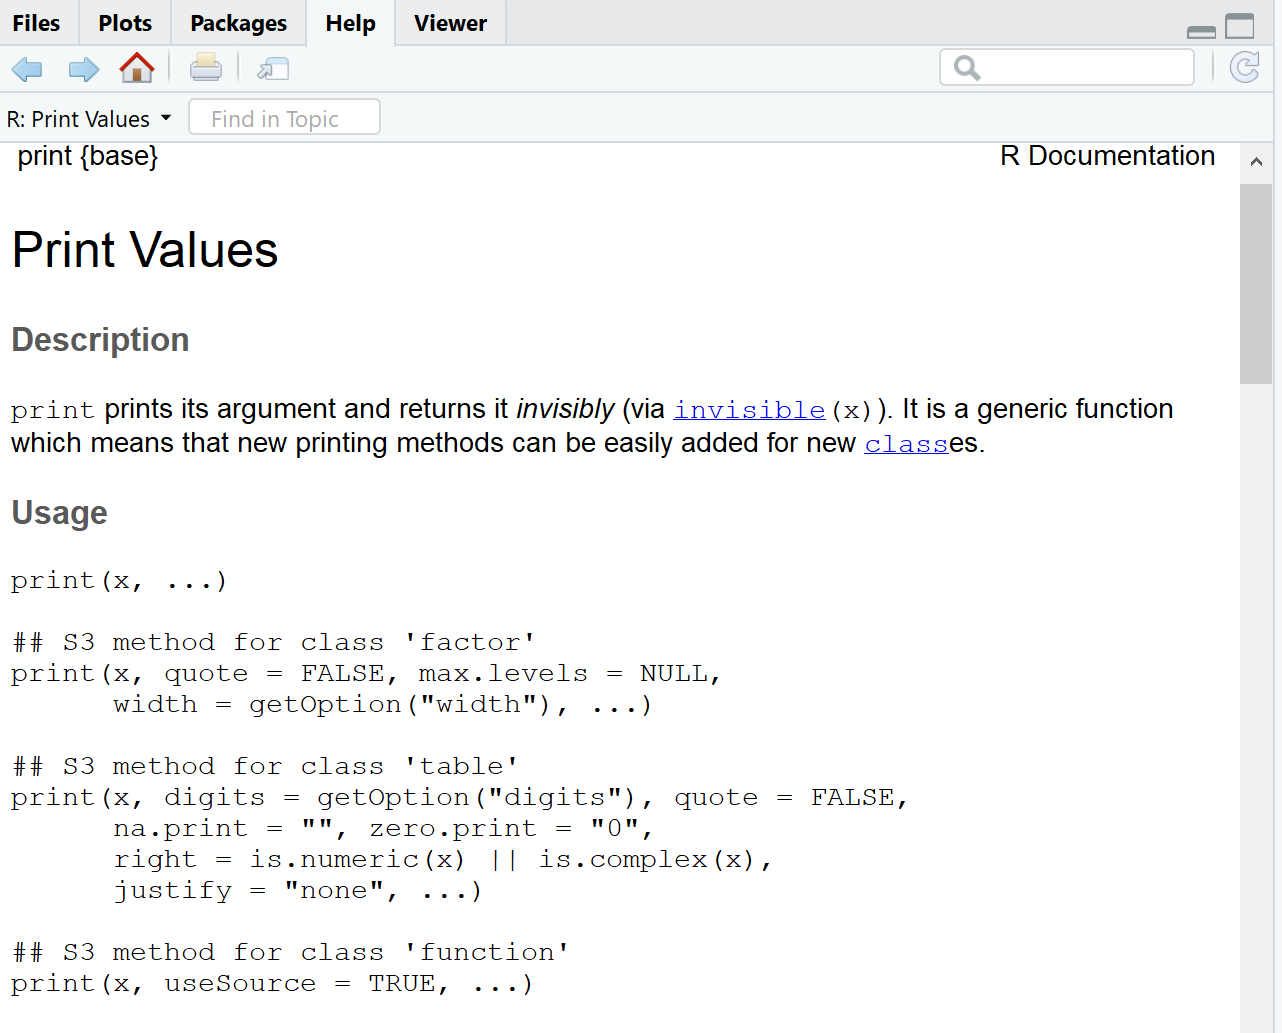
\includegraphics[width=0.5\linewidth]{/home/shulai/Insync/shulai@iu.edu/Google Drive/CAIDE Lab/R-tt/pics/print_exp}

Use single quotes to get help on operators

\begin{Shaded}
\begin{Highlighting}[]
\NormalTok{?}\StringTok{`}\DataTypeTok{:}\StringTok{`}
\end{Highlighting}
\end{Shaded}

These helping information in the picture above will show up on the
sidebar of R studio

\hypertarget{args-view-arguments-of-function}{%
\subsubsection{``args'': View arguments of
function}\label{args-view-arguments-of-function}}

To view the list of possible arguments a function can have use `args'

\begin{Shaded}
\begin{Highlighting}[]
\KeywordTok{args}\NormalTok{(png) }\CommentTok{#png is a function to export graph as png in your computer}
\end{Highlighting}
\end{Shaded}

\begin{verbatim}
## function (filename = "Rplot%03d.png", width = 480, height = 480, 
##     units = "px", pointsize = 12, bg = "white", res = NA, ..., 
##     type = c("cairo", "cairo-png", "Xlib", "quartz"), antialias) 
## NULL
\end{verbatim}

\hypertarget{view-the-whole-function}{%
\subsubsection{View the whole function}\label{view-the-whole-function}}

To see the whole function: type in the function name without ``()''
followed

\begin{Shaded}
\begin{Highlighting}[]
\NormalTok{var}
\end{Highlighting}
\end{Shaded}

\begin{verbatim}
## function (x, y = NULL, na.rm = FALSE, use) 
## {
##     if (missing(use)) 
##         use <- if (na.rm) 
##             "na.or.complete"
##         else "everything"
##     na.method <- pmatch(use, c("all.obs", "complete.obs", "pairwise.complete.obs", 
##         "everything", "na.or.complete"))
##     if (is.na(na.method)) 
##         stop("invalid 'use' argument")
##     if (is.data.frame(x)) 
##         x <- as.matrix(x)
##     else stopifnot(is.atomic(x))
##     if (is.data.frame(y)) 
##         y <- as.matrix(y)
##     else stopifnot(is.atomic(y))
##     .Call(C_cov, x, y, na.method, FALSE)
## }
## <bytecode: 0x556b26aac3f0>
## <environment: namespace:stats>
\end{verbatim}

\hypertarget{getset-working-dictionary-getwd-setwd}{%
\subsubsection{Get/set Working dictionary: ``getwd()''
``setwd()''}\label{getset-working-dictionary-getwd-setwd}}

Get current working dictionary:

\begin{Shaded}
\begin{Highlighting}[]
\KeywordTok{getwd}\NormalTok{()}
\end{Highlighting}
\end{Shaded}

\begin{verbatim}
## [1] "/home/shulai/Insync/shulai@iu.edu/Google Drive/CAIDE Lab/R-tt"
\end{verbatim}

Set current working dictionary:

\begin{Shaded}
\begin{Highlighting}[]
\KeywordTok{setwd}\NormalTok{(}\StringTok{"C:/Users/naszh/Desktop"}\NormalTok{)}
\end{Highlighting}
\end{Shaded}

As we started, (e.x.: a=c(1,2,\ldots{})) is a way to combine elelments
and create vectors. There also are other ways to create vectors:

\hypertarget{vector-or-array}{%
\subsection{vector or array}\label{vector-or-array}}

Create vector or array

\begin{Shaded}
\begin{Highlighting}[]
\NormalTok{x=}\KeywordTok{vector}\NormalTok{()}
\NormalTok{x[}\DecValTok{3}\NormalTok{]=}\DecValTok{10}
\NormalTok{x}
\end{Highlighting}
\end{Shaded}

\begin{verbatim}
## [1] NA NA 10
\end{verbatim}

\begin{Shaded}
\begin{Highlighting}[]
\NormalTok{y=}\KeywordTok{array}\NormalTok{()}
\NormalTok{y[}\DecValTok{4}\NormalTok{]=}\DecValTok{1}
\NormalTok{y}
\end{Highlighting}
\end{Shaded}

\begin{verbatim}
## [1] NA NA NA  1
\end{verbatim}

Difference between array and vector is that array can have more
dimensions than vector:

\begin{Shaded}
\begin{Highlighting}[]
\KeywordTok{array}\NormalTok{(}\DataTypeTok{dim=}\KeywordTok{c}\NormalTok{(}\DecValTok{1}\NormalTok{,}\DecValTok{2}\NormalTok{))}
\end{Highlighting}
\end{Shaded}

\begin{verbatim}
##      [,1] [,2]
## [1,]   NA   NA
\end{verbatim}

dim stands for dimension at here.

\hypertarget{assign-names-for-a-vector-or-array}{%
\subsubsection{Assign names for a vector or
array}\label{assign-names-for-a-vector-or-array}}

Vectors can have names for each element, and array can have column names
and row names

\begin{Shaded}
\begin{Highlighting}[]
\NormalTok{x=}\DecValTok{1}\OperatorTok{:}\DecValTok{10} \CommentTok{#x become a vector}
\KeywordTok{names}\NormalTok{(x)=}\KeywordTok{paste}\NormalTok{(}\StringTok{"X"}\NormalTok{,}\DecValTok{1}\OperatorTok{:}\DecValTok{10}\NormalTok{,}\DataTypeTok{sep=}\StringTok{""}\NormalTok{)}
\NormalTok{x}
\end{Highlighting}
\end{Shaded}

\begin{verbatim}
##  X1  X2  X3  X4  X5  X6  X7  X8  X9 X10 
##   1   2   3   4   5   6   7   8   9  10
\end{verbatim}

\begin{Shaded}
\begin{Highlighting}[]
\NormalTok{y=}\KeywordTok{array}\NormalTok{(}\DecValTok{2}\OperatorTok{:}\DecValTok{3}\NormalTok{,}\DataTypeTok{dim=}\KeywordTok{c}\NormalTok{(}\DecValTok{1}\NormalTok{,}\DecValTok{2}\NormalTok{))}
\KeywordTok{colnames}\NormalTok{(y)=}\KeywordTok{c}\NormalTok{(}\StringTok{"col1"}\NormalTok{,}\StringTok{"col2"}\NormalTok{) }\CommentTok{#define column names}
\KeywordTok{rownames}\NormalTok{(y)=}\StringTok{"row1"} \CommentTok{#define row names}
\NormalTok{y}
\end{Highlighting}
\end{Shaded}

\begin{verbatim}
##      col1 col2
## row1    2    3
\end{verbatim}

\hypertarget{call-elements-in-vector-or-array}{%
\subsubsection{Call elements in vector or
array}\label{call-elements-in-vector-or-array}}

call by names (use x and y value from above)

\begin{Shaded}
\begin{Highlighting}[]
\NormalTok{x[}\StringTok{"X1"}\NormalTok{] }\CommentTok{#don't forget to add " " on the name inside []}
\end{Highlighting}
\end{Shaded}

\begin{verbatim}
## X1 
##  1
\end{verbatim}

\begin{Shaded}
\begin{Highlighting}[]
\NormalTok{y[}\StringTok{"row1"}\NormalTok{,}\StringTok{"col1"}\NormalTok{]}
\end{Highlighting}
\end{Shaded}

\begin{verbatim}
## [1] 2
\end{verbatim}

Call by index number

\begin{Shaded}
\begin{Highlighting}[]
\CommentTok{#vector:}
\NormalTok{x=}\DecValTok{1}\OperatorTok{:}\DecValTok{10}
\NormalTok{x}
\end{Highlighting}
\end{Shaded}

\begin{verbatim}
##  [1]  1  2  3  4  5  6  7  8  9 10
\end{verbatim}

\begin{Shaded}
\begin{Highlighting}[]
\NormalTok{x[}\DecValTok{1}\NormalTok{]}
\end{Highlighting}
\end{Shaded}

\begin{verbatim}
## [1] 1
\end{verbatim}

\begin{Shaded}
\begin{Highlighting}[]
\NormalTok{x[}\DecValTok{1}\OperatorTok{:}\DecValTok{2}\NormalTok{]}
\end{Highlighting}
\end{Shaded}

\begin{verbatim}
## [1] 1 2
\end{verbatim}

\begin{Shaded}
\begin{Highlighting}[]
\CommentTok{#array:}
\NormalTok{y=}\KeywordTok{array}\NormalTok{(}\DecValTok{1}\OperatorTok{:}\DecValTok{20}\NormalTok{,}\DataTypeTok{dim=}\KeywordTok{c}\NormalTok{(}\DecValTok{4}\NormalTok{,}\DecValTok{5}\NormalTok{))}
\NormalTok{y}
\end{Highlighting}
\end{Shaded}

\begin{verbatim}
##      [,1] [,2] [,3] [,4] [,5]
## [1,]    1    5    9   13   17
## [2,]    2    6   10   14   18
## [3,]    3    7   11   15   19
## [4,]    4    8   12   16   20
\end{verbatim}

\begin{Shaded}
\begin{Highlighting}[]
\NormalTok{y[}\DecValTok{2}\NormalTok{,}\DecValTok{3}\NormalTok{] }\CommentTok{#row2, column 3}
\end{Highlighting}
\end{Shaded}

\begin{verbatim}
## [1] 10
\end{verbatim}

\begin{Shaded}
\begin{Highlighting}[]
\NormalTok{y[}\DecValTok{2}\NormalTok{, ] }\CommentTok{#present row 2}
\end{Highlighting}
\end{Shaded}

\begin{verbatim}
## [1]  2  6 10 14 18
\end{verbatim}

\hypertarget{select-only-certain-things-in-the-array}{%
\subsubsection{Select only certain things in the
array}\label{select-only-certain-things-in-the-array}}

\begin{Shaded}
\begin{Highlighting}[]
\NormalTok{x=}\DecValTok{1}\OperatorTok{:}\DecValTok{10}
\NormalTok{x[x}\OperatorTok{>}\DecValTok{5}\NormalTok{]}
\end{Highlighting}
\end{Shaded}

\begin{verbatim}
## [1]  6  7  8  9 10
\end{verbatim}

``x\textgreater{}5'' is a logical statement and give an array of logical
vlaues:

\begin{Shaded}
\begin{Highlighting}[]
\NormalTok{x}\OperatorTok{>}\DecValTok{5}
\end{Highlighting}
\end{Shaded}

\begin{verbatim}
##  [1] FALSE FALSE FALSE FALSE FALSE  TRUE  TRUE  TRUE  TRUE  TRUE
\end{verbatim}

This logical value array can be put into

\#\#Dataframe

create dataframe:

\begin{Shaded}
\begin{Highlighting}[]
\NormalTok{d =}\StringTok{ }\KeywordTok{data.frame}\NormalTok{(}\StringTok{"Feature1"}\NormalTok{ =}\StringTok{ }\KeywordTok{c}\NormalTok{(}\DecValTok{1}\NormalTok{,}\DecValTok{10}\NormalTok{,}\KeywordTok{rep}\NormalTok{(}\DecValTok{12}\NormalTok{,}\DecValTok{2}\NormalTok{)))}
\NormalTok{d}
\end{Highlighting}
\end{Shaded}

\begin{verbatim}
##   Feature1
## 1        1
## 2       10
## 3       12
## 4       12
\end{verbatim}

Call a column:

\begin{Shaded}
\begin{Highlighting}[]
\NormalTok{d}\OperatorTok{$}\NormalTok{Feature1}
\end{Highlighting}
\end{Shaded}

\begin{verbatim}
## [1]  1 10 12 12
\end{verbatim}

Add a column:

\begin{Shaded}
\begin{Highlighting}[]
\NormalTok{d =}\StringTok{ }\KeywordTok{cbind}\NormalTok{(d, }\StringTok{"Feature2"}\NormalTok{ =}\StringTok{ }\KeywordTok{c}\NormalTok{(}\DecValTok{10}\NormalTok{,}\DecValTok{29}\NormalTok{,}\DecValTok{9}\NormalTok{,}\DecValTok{2}\NormalTok{)) }\CommentTok{#cbind stand for column bind;}
    \CommentTok{#similarly, rbind is for row bind. }
\NormalTok{d}
\end{Highlighting}
\end{Shaded}

\begin{verbatim}
##   Feature1 Feature2
## 1        1       10
## 2       10       29
## 3       12        9
## 4       12        2
\end{verbatim}

\#\#Ploting

\hypertarget{plot}{%
\subsubsection{``plot''}\label{plot}}

You can plot data using the function `plot'

\begin{Shaded}
\begin{Highlighting}[]
\NormalTok{x =}\StringTok{ }\DecValTok{1}\OperatorTok{:}\DecValTok{10}\NormalTok{;y=}\DecValTok{2}\OperatorTok{:}\DecValTok{11}
\KeywordTok{plot}\NormalTok{(x,y)}
\end{Highlighting}
\end{Shaded}

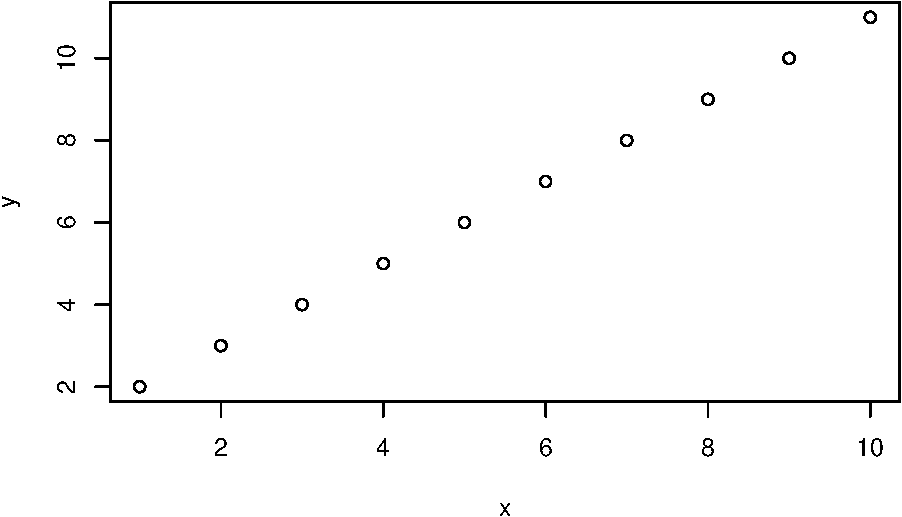
\includegraphics{tutorial_files/figure-latex/unnamed-chunk-32-1.pdf}

\hypertarget{export-plot-pdf-png}{%
\subsubsection{Export plot: ``pdf'',
``png''}\label{export-plot-pdf-png}}

Export plot as a pdf (or other formats).

\begin{Shaded}
\begin{Highlighting}[]
\KeywordTok{pdf}\NormalTok{(}\DataTypeTok{file=}\StringTok{"homework1_plot2.pdf"}\NormalTok{, }\DataTypeTok{height=}\DecValTok{3}\NormalTok{, }\DataTypeTok{width=}\DecValTok{3}\NormalTok{)}
\KeywordTok{plot}\NormalTok{(y,x)}
\KeywordTok{plot}\NormalTok{(x,x)}
\KeywordTok{dev.off}\NormalTok{()}
\end{Highlighting}
\end{Shaded}

\begin{verbatim}
## pdf 
##   2
\end{verbatim}

\begin{Shaded}
\begin{Highlighting}[]
  \CommentTok{#Run these functions together}
  \CommentTok{#the first commend "pdf" startsthe graphics device to pdf, }
  \CommentTok{#and the following graphics would be produced in the pdf  }
  \CommentTok{#When finish plotting, use dev,off to turns off the connection to the graphical device.}
  \CommentTok{#The file will show up in whatever your current working directory is.}
\end{Highlighting}
\end{Shaded}

\hypertarget{change-font-size-plot-lwd}{%
\subsubsection{Change font size: ``plot(\ldots{} , lwd=
)''}\label{change-font-size-plot-lwd}}

Use larger font for axis labels

\begin{Shaded}
\begin{Highlighting}[]
\KeywordTok{plot}\NormalTok{(x, y, }\DataTypeTok{type=}\StringTok{'l'}\NormalTok{, }\DataTypeTok{lwd=}\DecValTok{8}\NormalTok{)}
\end{Highlighting}
\end{Shaded}

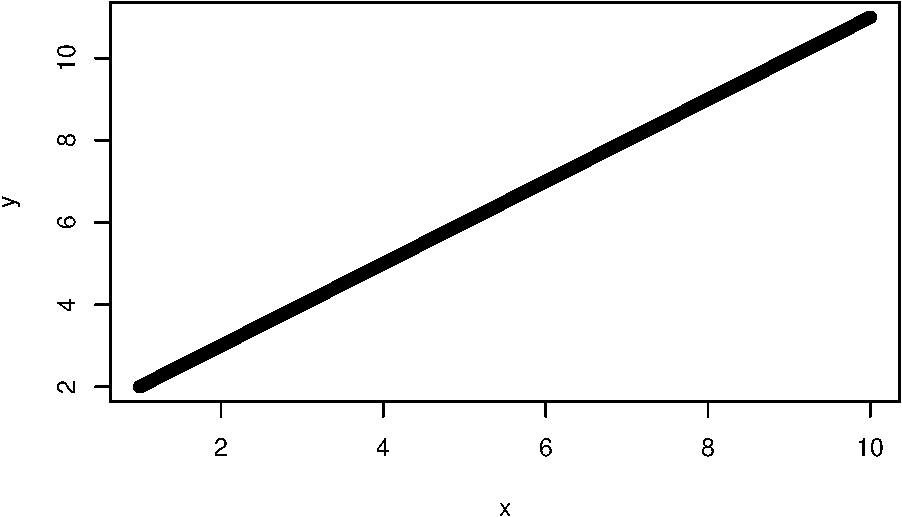
\includegraphics[width=0.5\linewidth]{tutorial_files/figure-latex/unnamed-chunk-34-1}

\begin{Shaded}
\begin{Highlighting}[]
\KeywordTok{plot}\NormalTok{(x, y, }\DataTypeTok{type=}\StringTok{'l'}\NormalTok{, }\DataTypeTok{lwd=}\DecValTok{3}\NormalTok{)}
\end{Highlighting}
\end{Shaded}

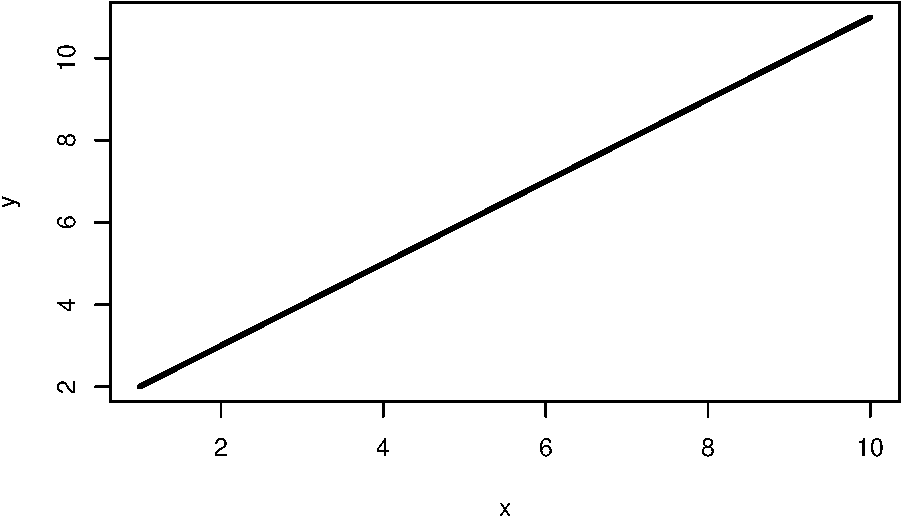
\includegraphics[width=0.5\linewidth]{tutorial_files/figure-latex/unnamed-chunk-34-2}

\hypertarget{change-font-color-plot-col}{%
\subsubsection{Change font color: ``plot(\ldots{} , col=
)''}\label{change-font-color-plot-col}}

\begin{Shaded}
\begin{Highlighting}[]
\KeywordTok{plot}\NormalTok{(x, y, }\DataTypeTok{type=}\StringTok{'l'}\NormalTok{, }\DataTypeTok{lwd=}\DecValTok{8}\NormalTok{, }\DataTypeTok{col=}\StringTok{'blue'}\NormalTok{)}
\end{Highlighting}
\end{Shaded}

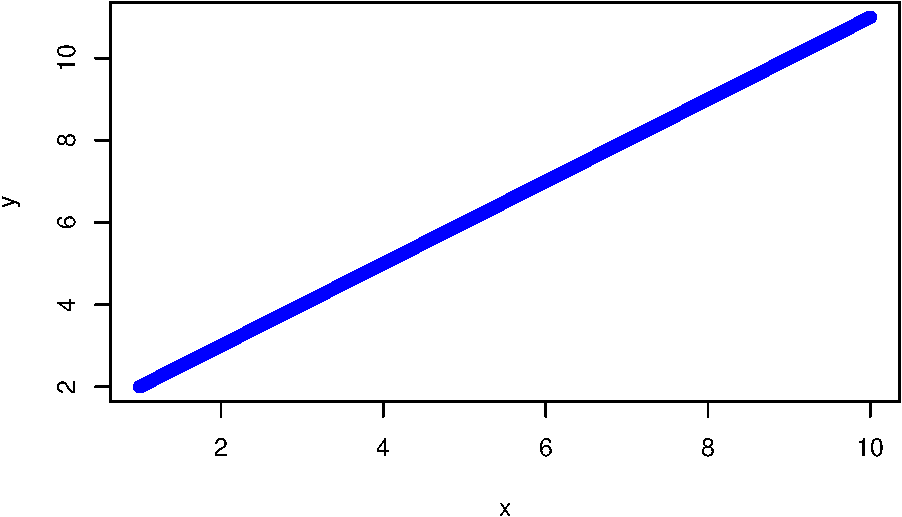
\includegraphics[width=0.5\linewidth]{tutorial_files/figure-latex/unnamed-chunk-35-1}

\hypertarget{change-type-of-plot-plot-type}{%
\subsubsection{Change type of plot: ``plot(\ldots{}, type=
)''}\label{change-type-of-plot-plot-type}}

\begin{Shaded}
\begin{Highlighting}[]
\KeywordTok{plot}\NormalTok{(x, y, }\DataTypeTok{type=}\StringTok{'l'}\NormalTok{) }\CommentTok{# "l" for lines}
\end{Highlighting}
\end{Shaded}

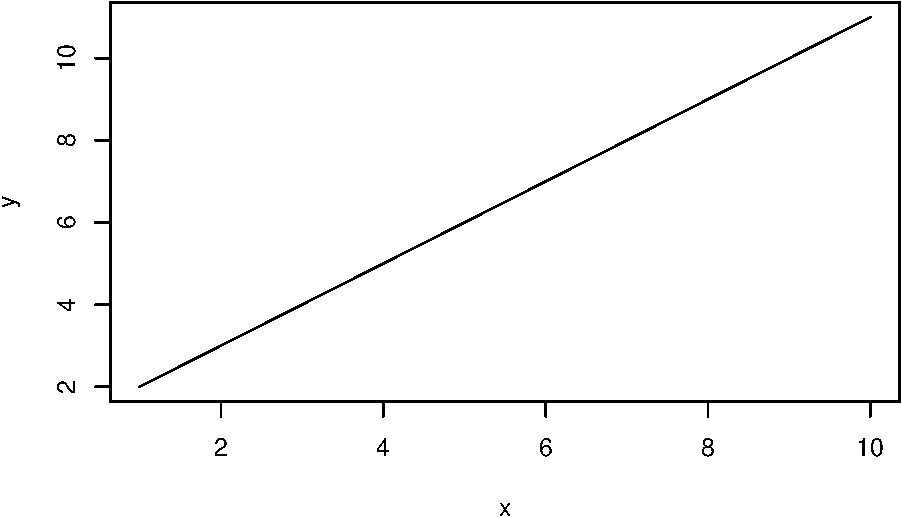
\includegraphics[width=0.5\linewidth]{tutorial_files/figure-latex/unnamed-chunk-36-1}

\begin{Shaded}
\begin{Highlighting}[]
\KeywordTok{plot}\NormalTok{(x, y, }\DataTypeTok{type=}\StringTok{'p'}\NormalTok{) }\CommentTok{# "p" for points}
\end{Highlighting}
\end{Shaded}

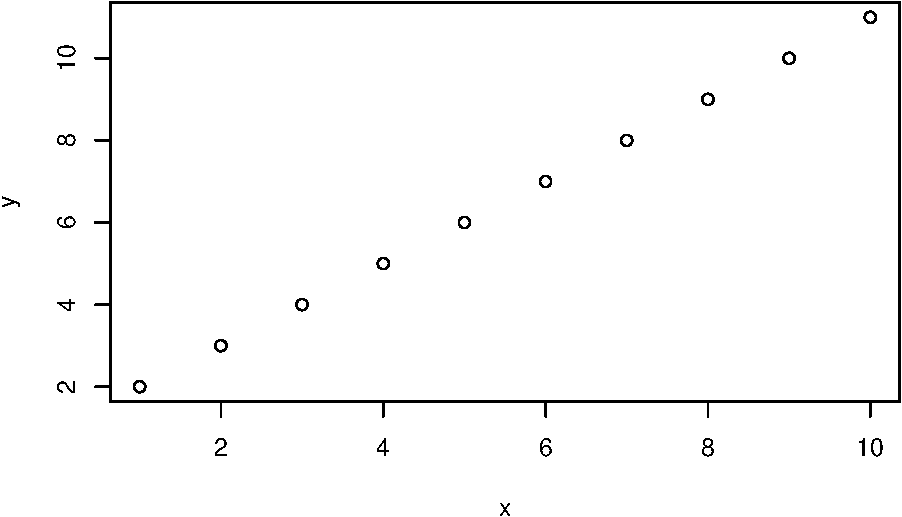
\includegraphics[width=0.5\linewidth]{tutorial_files/figure-latex/unnamed-chunk-36-2}

\begin{Shaded}
\begin{Highlighting}[]
\KeywordTok{plot}\NormalTok{(x, y, }\DataTypeTok{type=}\StringTok{'b'}\NormalTok{) }\CommentTok{# "b" for both}
\end{Highlighting}
\end{Shaded}

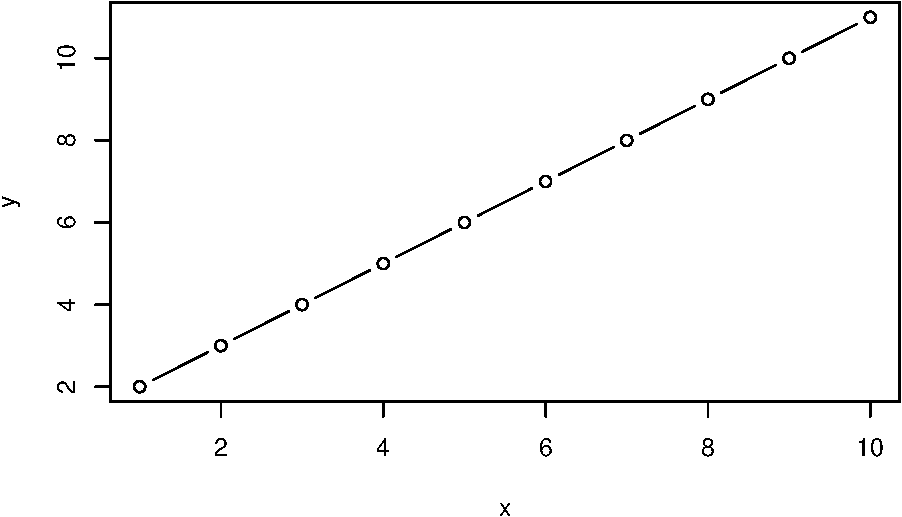
\includegraphics[width=0.5\linewidth]{tutorial_files/figure-latex/unnamed-chunk-36-3}
More types usage see ``?plot''

\hypertarget{change-title-lab-names}{%
\subsubsection{Change title/ lab names}\label{change-title-lab-names}}

\begin{Shaded}
\begin{Highlighting}[]
\KeywordTok{plot}\NormalTok{(x, y, }\DataTypeTok{type=}\StringTok{'l'}\NormalTok{,}\DataTypeTok{xlab=}\StringTok{"Time"}\NormalTok{,}\DataTypeTok{ylab=}\StringTok{"Grade"}\NormalTok{,}\DataTypeTok{main=}\StringTok{"Time-Grade"}\NormalTok{,}\DataTypeTok{sub=}\StringTok{"Plot 1"}\NormalTok{)}
\end{Highlighting}
\end{Shaded}

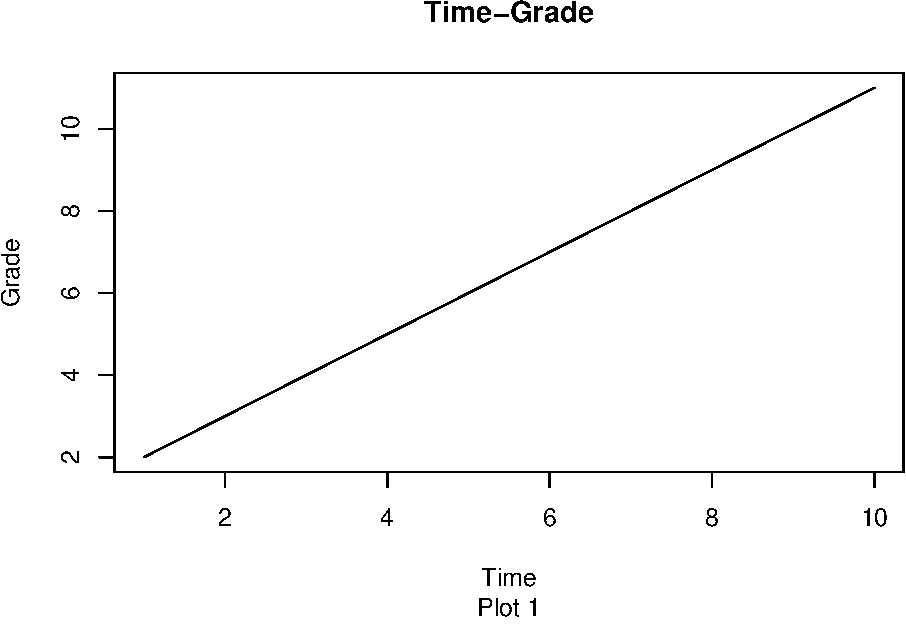
\includegraphics[width=0.5\linewidth]{tutorial_files/figure-latex/unnamed-chunk-37-1}

\end{document}
